    
    
    

    
    \hypertarget{euler-method-for-solving-first-order-differential-equations}{%
\section{Euler method for solving first-order differential
equations}\label{euler-method-for-solving-first-order-differential-equations}}

    The Euler method is a numerical algorithm for solving ordinary
differential equations given an initial value.

Given an initial value, the method works by evaluating the function
\(f(x)\) at a point \(x = x_{n+1}\) using straight line approximation
with slope \(f'(x)\) at \(x = x_n\), where the step,
\(h = x_{n+1} - x_n\).

Using the first principle of derivatives,
\[f'(x_0) = \lim_{h \rightarrow 0}  \frac{f(x_0 + h) - f(x_0)}{h}\]
Therfore, if \(h\) is small enough,
\[f(x_0 + h) \approx f(x_0) + h \cdot f'(x_0)\]

    Another possible explanation of this approximation, can originate from
the Taylor expansion,
\[f(x_0 + h) = f(x_0) + h \cdot f'(x_0) + h^2 \cdot f''(x_0) + h^3 \cdot f'''(x_0) + \dots\]

Since \(h << 1\), ignoring the higher order terms the approximation
becomes, \[f(x_0 + h) \approx f(x_0) + h \cdot f'(x_0)\]

Then the function \(f(x)\) at a generic point \(x_n\) can be
approximated using, \[f(x_n) \approx f(x_{n-1}) + h \cdot f'(x_{n-1})\]

The intial value of \(f(x)\) at \(x = x_0\) must be provided, which will
be the starting point for the Euler method algorithm. This will
eliminate the constant we would have got from solving the first-order
differential equation.

    An Illustration of the Euler method is given below,

\begin{figure}
\centering
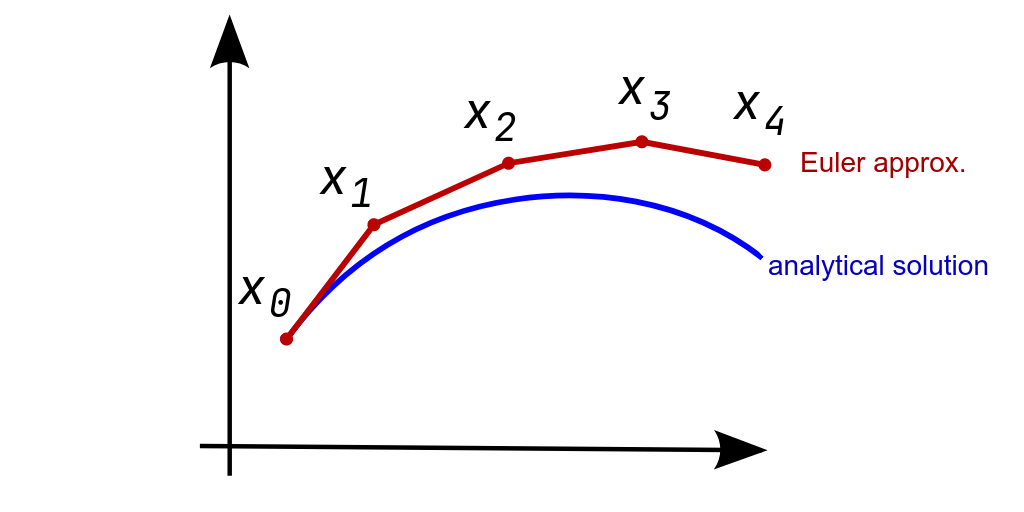
\includegraphics{resources/euler-1.png}
\caption{resources/euler-1.png}
\end{figure}

    \hypertarget{code}{%
\subsection{Code}\label{code}}

    \begin{tcolorbox}[breakable, size=fbox, boxrule=1pt, pad at break*=1mm,colback=cellbackground, colframe=cellborder]
\prompt{In}{incolor}{1}{\boxspacing}
\begin{Verbatim}[commandchars=\\\{\}]
\PY{k+kn}{from} \PY{n+nn}{numpy} \PY{k+kn}{import} \PY{n}{cos}\PY{p}{,} \PY{n}{empty}\PY{p}{,} \PY{n}{exp}\PY{p}{,} \PY{n}{pi}\PY{p}{,} \PY{n}{sin}
\PY{k+kn}{from} \PY{n+nn}{matplotlib} \PY{k+kn}{import} \PY{n}{pyplot} \PY{k}{as} \PY{n}{plt}

\PY{c+c1}{\PYZsh{} Default configuaration for matplotlib}
\PY{n}{plt}\PY{o}{.}\PY{n}{style}\PY{o}{.}\PY{n}{use}\PY{p}{(}\PY{p}{[}\PY{l+s+s1}{\PYZsq{}}\PY{l+s+s1}{science}\PY{l+s+s1}{\PYZsq{}}\PY{p}{,} \PY{l+s+s1}{\PYZsq{}}\PY{l+s+s1}{ieee}\PY{l+s+s1}{\PYZsq{}}\PY{p}{]}\PY{p}{)}
\PY{n}{plt}\PY{o}{.}\PY{n}{rcParams}\PY{p}{[}\PY{l+s+s2}{\PYZdq{}}\PY{l+s+s2}{figure.figsize}\PY{l+s+s2}{\PYZdq{}}\PY{p}{]} \PY{o}{=} \PY{p}{(}\PY{l+m+mi}{10}\PY{p}{,} \PY{l+m+mi}{5}\PY{p}{)}
\end{Verbatim}
\end{tcolorbox}

    \begin{tcolorbox}[breakable, size=fbox, boxrule=1pt, pad at break*=1mm,colback=cellbackground, colframe=cellborder]
\prompt{In}{incolor}{2}{\boxspacing}
\begin{Verbatim}[commandchars=\\\{\}]
\PY{c+c1}{\PYZsh{} Function to generate `n` evenly spaced points between limits `a` and `b`}
\PY{k}{def} \PY{n+nf}{generate\PYZus{}points}\PY{p}{(}\PY{n}{a}\PY{p}{,} \PY{n}{b}\PY{p}{,} \PY{n}{h}\PY{p}{)}\PY{p}{:}

    \PY{c+c1}{\PYZsh{} Calculating the number of points}
    \PY{n}{n} \PY{o}{=} \PY{n+nb}{int}\PY{p}{(}\PY{p}{(}\PY{p}{(}\PY{n}{b} \PY{o}{\PYZhy{}} \PY{n}{a}\PY{p}{)} \PY{o}{/} \PY{n}{h}\PY{p}{)} \PY{o}{+} \PY{l+m+mi}{1}\PY{p}{)}

    \PY{c+c1}{\PYZsh{} Creating an empty array to store the points}
    \PY{n}{points} \PY{o}{=} \PY{n}{empty}\PY{p}{(}\PY{n}{n}\PY{p}{)}

    \PY{c+c1}{\PYZsh{} Generating the points}
    \PY{k}{for} \PY{n}{i} \PY{o+ow}{in} \PY{n+nb}{range}\PY{p}{(}\PY{n}{n}\PY{p}{)}\PY{p}{:}
        \PY{n}{points}\PY{p}{[}\PY{n}{i}\PY{p}{]} \PY{o}{=} \PY{n}{a}
        \PY{n}{a} \PY{o}{+}\PY{o}{=} \PY{n}{h}

    \PY{k}{return} \PY{n}{points}
\end{Verbatim}
\end{tcolorbox}

    \begin{tcolorbox}[breakable, size=fbox, boxrule=1pt, pad at break*=1mm,colback=cellbackground, colframe=cellborder]
\prompt{In}{incolor}{3}{\boxspacing}
\begin{Verbatim}[commandchars=\\\{\}]
\PY{c+c1}{\PYZsh{} Code for solving first\PYZhy{}order ordinary differential equations using Euler method}
\PY{k}{def} \PY{n+nf}{solve\PYZus{}euler}\PY{p}{(}\PY{n}{y\PYZus{}prime}\PY{p}{,} \PY{n}{x\PYZus{}i}\PY{p}{,} \PY{n}{x\PYZus{}f}\PY{p}{,} \PY{n}{y\PYZus{}i}\PY{p}{,} \PY{n}{h}\PY{p}{)}\PY{p}{:}

    \PY{c+c1}{\PYZsh{} Generating equispaced points}
    \PY{n}{x} \PY{o}{=} \PY{n}{generate\PYZus{}points}\PY{p}{(}\PY{n}{x\PYZus{}i}\PY{p}{,} \PY{n}{x\PYZus{}f}\PY{p}{,} \PY{n}{h}\PY{p}{)}

    \PY{c+c1}{\PYZsh{} Creating a array to store `y`}
    \PY{n}{y} \PY{o}{=} \PY{n}{empty}\PY{p}{(}\PY{n}{x}\PY{o}{.}\PY{n}{size}\PY{p}{)}

    \PY{c+c1}{\PYZsh{} Initialising `y` with initial value}
    \PY{n}{y}\PY{p}{[}\PY{l+m+mi}{0}\PY{p}{]} \PY{o}{=} \PY{n}{y\PYZus{}i}

    \PY{c+c1}{\PYZsh{} Evaluating the function `y` at the remaining points}
    \PY{k}{for} \PY{n}{i} \PY{o+ow}{in} \PY{n+nb}{range}\PY{p}{(}\PY{l+m+mi}{1}\PY{p}{,} \PY{n}{x}\PY{o}{.}\PY{n}{size}\PY{p}{)}\PY{p}{:}
        \PY{n}{y}\PY{p}{[}\PY{n}{i}\PY{p}{]} \PY{o}{=} \PY{n}{y}\PY{p}{[}\PY{n}{i}\PY{o}{\PYZhy{}}\PY{l+m+mi}{1}\PY{p}{]} \PY{o}{+} \PY{n}{h} \PY{o}{*} \PY{n}{y\PYZus{}prime}\PY{p}{(}\PY{n}{x}\PY{p}{[}\PY{n}{i}\PY{p}{]}\PY{p}{,} \PY{n}{y}\PY{p}{[}\PY{n}{i}\PY{o}{\PYZhy{}}\PY{l+m+mi}{1}\PY{p}{]}\PY{p}{)}

    \PY{k}{return} \PY{n}{x}\PY{p}{,} \PY{n}{y}
\end{Verbatim}
\end{tcolorbox}

    \hypertarget{examples}{%
\subsection{Examples}\label{examples}}

    \hypertarget{fracdydx-y}{%
\subsubsection{\texorpdfstring{\[\frac{dy}{dx} = y\]}{\textbackslash frac\{dy\}\{dx\} = y}}\label{fracdydx-y}}

    \begin{tcolorbox}[breakable, size=fbox, boxrule=1pt, pad at break*=1mm,colback=cellbackground, colframe=cellborder]
\prompt{In}{incolor}{4}{\boxspacing}
\begin{Verbatim}[commandchars=\\\{\}]
\PY{k}{def} \PY{n+nf}{y\PYZus{}prime}\PY{p}{(}\PY{n}{x}\PY{p}{,} \PY{n}{y}\PY{p}{)}\PY{p}{:}
    \PY{k}{return} \PY{n}{y}


\PY{n}{x\PYZus{}i} \PY{o}{=} \PY{l+m+mi}{0}
\PY{n}{x\PYZus{}f} \PY{o}{=} \PY{l+m+mi}{5}
\PY{n}{y\PYZus{}i} \PY{o}{=} \PY{l+m+mi}{1}
\PY{n}{h} \PY{o}{=} \PY{l+m+mf}{0.1}
\end{Verbatim}
\end{tcolorbox}

    \begin{tcolorbox}[breakable, size=fbox, boxrule=1pt, pad at break*=1mm,colback=cellbackground, colframe=cellborder]
\prompt{In}{incolor}{5}{\boxspacing}
\begin{Verbatim}[commandchars=\\\{\}]
\PY{c+c1}{\PYZsh{} Euler approximation}
\PY{n}{points}\PY{p}{,} \PY{n}{y\PYZus{}euler} \PY{o}{=} \PY{n}{solve\PYZus{}euler}\PY{p}{(}\PY{n}{y\PYZus{}prime}\PY{p}{,} \PY{n}{x\PYZus{}i}\PY{p}{,} \PY{n}{x\PYZus{}f}\PY{p}{,} \PY{n}{y\PYZus{}i}\PY{p}{,} \PY{n}{h}\PY{p}{)}

\PY{c+c1}{\PYZsh{} Analytical solution}
\PY{n}{y\PYZus{}analytical} \PY{o}{=} \PY{n}{exp}\PY{p}{(}\PY{n}{points}\PY{p}{)}
\end{Verbatim}
\end{tcolorbox}

    \begin{tcolorbox}[breakable, size=fbox, boxrule=1pt, pad at break*=1mm,colback=cellbackground, colframe=cellborder]
\prompt{In}{incolor}{6}{\boxspacing}
\begin{Verbatim}[commandchars=\\\{\}]
\PY{n}{plt}\PY{o}{.}\PY{n}{plot}\PY{p}{(}\PY{n}{points}\PY{p}{,} \PY{n}{y\PYZus{}euler}\PY{p}{,} \PY{n}{label}\PY{o}{=}\PY{l+s+s2}{\PYZdq{}}\PY{l+s+s2}{euler approximation}\PY{l+s+s2}{\PYZdq{}}\PY{p}{)}
\PY{n}{plt}\PY{o}{.}\PY{n}{plot}\PY{p}{(}\PY{n}{points}\PY{p}{,} \PY{n}{y\PYZus{}analytical}\PY{p}{,} \PY{l+s+s1}{\PYZsq{}}\PY{l+s+s1}{.}\PY{l+s+s1}{\PYZsq{}}\PY{p}{,} \PY{n}{label}\PY{o}{=}\PY{l+s+s2}{\PYZdq{}}\PY{l+s+s2}{analytical solution (\PYZdl{}e\PYZca{}x\PYZdl{})}\PY{l+s+s2}{\PYZdq{}}\PY{p}{)}
\PY{n}{plt}\PY{o}{.}\PY{n}{legend}\PY{p}{(}\PY{p}{)}
\PY{n}{plt}\PY{o}{.}\PY{n}{show}\PY{p}{(}\PY{p}{)}
\end{Verbatim}
\end{tcolorbox}

    \begin{center}
    \adjustimage{max size={0.9\linewidth}{0.9\paperheight}}{9_Euler_method_for_solving_first_order_differential_equations_files/9_Euler_method_for_solving_first_order_differential_equations_12_0.png}
    \end{center}
    { \hspace*{\fill} \\}
    
    \hypertarget{fracdydx-sinx}{%
\subsubsection{\texorpdfstring{\[\frac{dy}{dx} = sin(x)\]}{\textbackslash frac\{dy\}\{dx\} = sin(x)}}\label{fracdydx-sinx}}

    \begin{tcolorbox}[breakable, size=fbox, boxrule=1pt, pad at break*=1mm,colback=cellbackground, colframe=cellborder]
\prompt{In}{incolor}{7}{\boxspacing}
\begin{Verbatim}[commandchars=\\\{\}]
\PY{k}{def} \PY{n+nf}{y\PYZus{}prime}\PY{p}{(}\PY{n}{x}\PY{p}{,} \PY{n}{y}\PY{p}{)}\PY{p}{:}
    \PY{k}{return} \PY{n}{sin}\PY{p}{(}\PY{n}{x}\PY{p}{)}


\PY{n}{x\PYZus{}i} \PY{o}{=} \PY{l+m+mi}{0}
\PY{n}{x\PYZus{}f} \PY{o}{=} \PY{l+m+mi}{2} \PY{o}{*} \PY{n}{pi}
\PY{n}{y\PYZus{}i} \PY{o}{=} \PY{o}{\PYZhy{}} \PY{l+m+mi}{1}
\PY{n}{h} \PY{o}{=} \PY{l+m+mf}{0.1}
\end{Verbatim}
\end{tcolorbox}

    \begin{tcolorbox}[breakable, size=fbox, boxrule=1pt, pad at break*=1mm,colback=cellbackground, colframe=cellborder]
\prompt{In}{incolor}{8}{\boxspacing}
\begin{Verbatim}[commandchars=\\\{\}]
\PY{c+c1}{\PYZsh{} Euler approximation}
\PY{n}{points}\PY{p}{,} \PY{n}{y\PYZus{}euler} \PY{o}{=} \PY{n}{solve\PYZus{}euler}\PY{p}{(}\PY{n}{y\PYZus{}prime}\PY{p}{,} \PY{n}{x\PYZus{}i}\PY{p}{,} \PY{n}{x\PYZus{}f}\PY{p}{,} \PY{n}{y\PYZus{}i}\PY{p}{,} \PY{n}{h}\PY{p}{)}

\PY{c+c1}{\PYZsh{} Analytical solution}
\PY{n}{y\PYZus{}analytical} \PY{o}{=} \PY{o}{\PYZhy{}}\PY{n}{cos}\PY{p}{(}\PY{n}{points}\PY{p}{)}
\end{Verbatim}
\end{tcolorbox}

    \begin{tcolorbox}[breakable, size=fbox, boxrule=1pt, pad at break*=1mm,colback=cellbackground, colframe=cellborder]
\prompt{In}{incolor}{9}{\boxspacing}
\begin{Verbatim}[commandchars=\\\{\}]
\PY{n}{plt}\PY{o}{.}\PY{n}{plot}\PY{p}{(}\PY{n}{points}\PY{p}{,} \PY{n}{y\PYZus{}euler}\PY{p}{,} \PY{n}{label}\PY{o}{=}\PY{l+s+s2}{\PYZdq{}}\PY{l+s+s2}{euler approximation}\PY{l+s+s2}{\PYZdq{}}\PY{p}{)}
\PY{n}{plt}\PY{o}{.}\PY{n}{plot}\PY{p}{(}\PY{n}{points}\PY{p}{,} \PY{n}{y\PYZus{}analytical}\PY{p}{,} \PY{l+s+s1}{\PYZsq{}}\PY{l+s+s1}{.}\PY{l+s+s1}{\PYZsq{}}\PY{p}{,} \PY{n}{label}\PY{o}{=}\PY{l+s+s2}{\PYZdq{}}\PY{l+s+s2}{analytical solution (\PYZdl{}cos(x)\PYZdl{})}\PY{l+s+s2}{\PYZdq{}}\PY{p}{)}
\PY{n}{plt}\PY{o}{.}\PY{n}{legend}\PY{p}{(}\PY{p}{)}
\PY{n}{plt}\PY{o}{.}\PY{n}{show}\PY{p}{(}\PY{p}{)}
\end{Verbatim}
\end{tcolorbox}

    \begin{center}
    \adjustimage{max size={0.9\linewidth}{0.9\paperheight}}{9_Euler_method_for_solving_first_order_differential_equations_files/9_Euler_method_for_solving_first_order_differential_equations_16_0.png}
    \end{center}
    { \hspace*{\fill} \\}
    

    % Add a bibliography block to the postdoc
    
    
    
